% The very first letter is a 2 line initial drop letter followed
% by the rest of the first word in caps.
% 
% form to use if the first word consists of a single letter:
% \IEEEPARstart{A}{demo} file is ....
% 
% form to use if you need the single drop letter followed by
% normal text (unknown if ever used by IEEE):
% \IEEEPARstart{A}{}demo file is ....
% 
% Some journals put the first two words in caps:
% \IEEEPARstart{T}{his demo} file is ....
% 
% Here we have the typical use of a "T" for an initial drop letter
% and "HIS" in caps to complete the first word.

\IEEEPARstart{N}{owadays} face recognition is becoming more and more important. People are being observed everywhere: surveillance monitoring, streets, shops, ATMs, social networks and general human-computer interaction\cite{Forensics}.

The human face is one of the most popular
characteristic which can be used in the biometric security system
to identify or verify a user. Face is an acceptable biometric
modality because it can be captured from a distance, even
without physical contact of the user being identified. Thus the
identification or verification does not require cooperation of the
user. Recognition systems based on human face are used for a
wide variety of applications, due to these benefits\cite{Occlusion&noise}.

Face recognition encounters many distractions like: partial occlusion, different angles (pitch, roll, yaw), lightning conditions (e.g. night vision). Usually all the computing has to be done under strict time requirements.

In the event of Boston marathon bombings,
images of the suspects taken from street surveillance cameras
aided the FBI to identify the suspects.\cite{NYTimes}

Face recognition includes the studies of automatically
identifying or verifying a person from an image or video
sequences. Face identification refers to determining the ID of
the person, given as a probe, from a large pool of candidates
in the gallery. Face verification or face authentication is the problem of deciding whether a given pair of images are
of the same person or not\cite{Forensics}.


\emph{Example of signifacance of patrial occlusion}
%%\title{Signifacance of patrial occlusion}
%%\subsection{\textbf{Signifacance of patrial occlusion}}
\begin{itemize}
	\item Eyes (occlusion of original image ~ 6\%)
	\item Eyebrows (occlusion of original image ~ 6\%)
	\item Mouth (occlusion of original image ~ 11\%)
	\item Eyes and nose (occlusion of original image ~ 9\%)
	\item Glasses (occlusion of original image ~ 15.5\%)
\end{itemize} 

\begin{figure}[ht]
	\centering		
	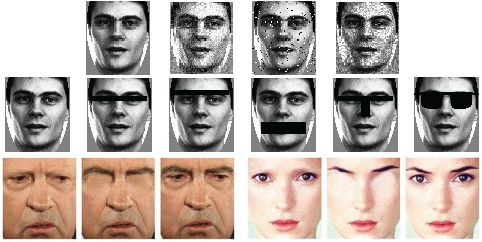
\includegraphics[width = 0.4\textwidth]{rsrc/faces.png}
	\caption{Different occuring distractions \cite{Occlusion&noise}.}
	\label{fig:Distractions}
\end{figure}
